\documentclass{article}
\usepackage[margin=1in]{geometry}
\usepackage{amsmath}
\usepackage{graphicx}
\usepackage{siunitx}
\usepackage{listings}
\usepackage{xcolor}
\usepackage{booktabs}
\usepackage{hyperref}
\definecolor{mygreen}{rgb}{0,0.6,0}
\definecolor{mygray}{rgb}{0.5,0.5,0.5}
\definecolor{mymauve}{rgb}{0.58,0,0.82}

\lstset{ %
  backgroundcolor=\color{white},   % choose the background color; you must add \usepackage{color} or \usepackage{xcolor}
  basicstyle=\scriptsize\ttfamily,    % the size of the fonts that are used for the code
  breakatwhitespace=false,         % sets if automatic breaks should only happen at whitespace
  breaklines=true,                 % sets automatic line breaking
  captionpos=b,                    % sets the caption-position to bottom
  commentstyle=\color{mygreen},    % comment style
  deletekeywords={},            % if you want to delete keywords from the given language
  escapeinside={\%*}{*)},          % if you want to add LaTeX within your code
  extendedchars=true,              % lets you use non-ASCII characters; for 8-bits encodings only, does not work with UTF-8
  frame=shadowbox,                    % adds a frame around the code
%  framexleftmarign=5mm,
  xleftmargin=10pt,
  xrightmargin=10pt,
  rulesepcolor=\color{gray},
  keywordstyle=\color{blue},       % keyword style
  language=Octave,                 % the language of the code
  morekeywords={*,...,fit,predint,export\_fig},            % if you want to add more keywords to the set
%  numbers=left,                    % where to put the line-numbers; possible values are (none, left, right)
  numbers=none,
  numbersep=5pt,                   % how far the line-numbers are from the code
  numberstyle=\tiny\color{mygray}, % the style that is used for the line-numbers
  rulecolor=\color{black},         % if not set, the frame-color may be changed on line-breaks within not-black text (e.g. comments (green here))
  showspaces=false,                % show spaces everywhere adding particular underscores; it overrides 'showstringspaces'
  showstringspaces=false,          % underline spaces within strings only
  showtabs=false,                  % show tabs within strings adding particular underscores
  stepnumber=1,                    % the step between two line-numbers. If it's 1, each line will be numbered
  stringstyle=\color{mymauve},     % string literal style
  tabsize=4,                       % sets default tabsize to 4 spaces
  caption=\lstname                   % show the filename of files included with \lstinputlisting; also try caption instead of title
}


\title{1.723 HW7}
\author{Sachith  Dunatunga}

\begin{document}
\newcommand{\deriv}[2]{\frac{\partial #1}{ \partial #2}}
\newcommand{\nderiv}[3]{\frac{\partial^{#3} #1}{ \partial #2^{#3}}}
\newcommand{\dx}[1]{\deriv{#1}{x}}
\newcommand{\taylorexpf}[3]{#1_{#2} + \left(#3 \right) \dx{#1}\biggr\rvert_{#2} + \frac{1}{2}\left(#3 \right)^2 \nderiv{#1}{x}{2}\biggr\rvert_{#2} + \frac{1}{6}\left(#3 \right)^3\nderiv{#1}{x}{3}\biggr\rvert_{#2} + \frac{1}{24}\left(#3 \right)^4\nderiv{#1}{x}{4}\biggr\rvert_{#2} + O(h^5)}
\maketitle

\section{Problem 1}
We are given the function $u(x) = \exp(ikx)$.
The deriviative of this function is $u'(x) = ik \exp(ikx)$, which can be written as $u'(x) = g_\infty(k) u(x)$ where $g_\infty(k) = ik$.
If we take the second order accurate centered finite difference first derivative, we can derive a function $g_2(k)$.
Writing the forumla for the differentiation, we begin with
\begin{align}
    u'_j &= \frac{1}{2h} \left( u(x_{j+1}) - u(x_{j-1}) \right) \\
    u'_j &= \frac{1}{2h} \left( \exp(ik(x_j + h)) - \exp(ik(x_j - h))\right) \\
    u'_j &= \frac{1}{2h} \left( \exp(ikh) - \exp(-ikh)\right) \exp(ikx_j)
\end{align}
for an arbitrary point $x_j$.
After some manipulation we obtain
\begin{align}
    g_2(k) = \frac{i}{h}\sin(kh).
\end{align}

Similarly, we can write the formula for the fourth order accurate centered finite difference approximation
\begin{align}
    u'_j &= \frac{1}{12h} \left( -u(x_{j+2}) + 8u(x_{j+1}) - 8u(x_{j-1}) + u(x_{j-2}) \right) \\
    u'_j &= \frac{1}{12h} \left( -\exp(ik(x+2h)) + 8\exp(ik(x+h)) - 8\exp(ik(x-h)) + \exp(ik(x-2h)) \right) \\
    u'_j &= \frac{1}{12h} \left( -\exp(i2kh) + 8\exp(ikh) - 8\exp(-ikh) + \exp(-i2kh) \right) \exp(ikx)
\end{align}
which can be rewritten as $u'_j = g_4(k) u_j$ where
\begin{align}
    g_2(k) = \frac{i}{6h}\left( 8\sin(kh) - \sin(2kh) \right).
\end{align}

Note that because of the grid spacing (which results in aliasing), the maxmium wavenumber in the discrete cases is given by $k = \pi / h$.

Plots of the imaginary component of these functions are shown in figure \ref{fig:p1}.
In the plots we have used a value of $h = 0.01$.
This means that in the discrete cases the maximum wavenumber is given by $100\pi$, and the range of our plots is trimmed accordingly.

\begin{figure}[!ht]
\centering
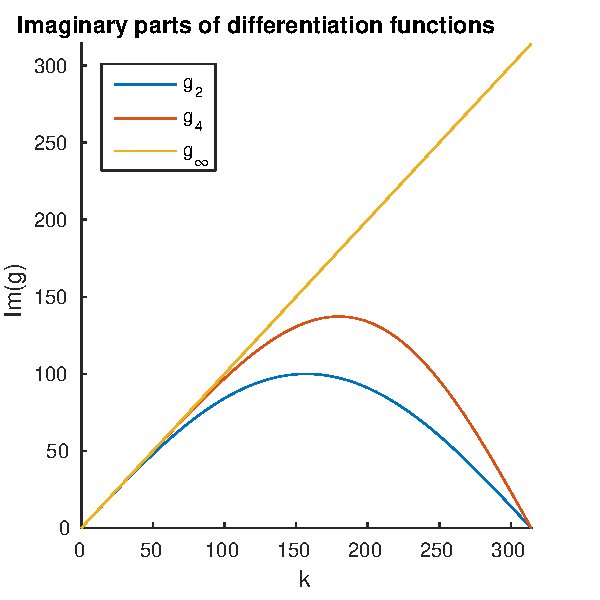
\includegraphics[scale=1.0]{p1.pdf}
\caption{Plots of the imaginary parts of $g_2(k), g_4(k)$, and $g_\infty(k)$. The spacing in the discrete cases is given by $h = 0.01$.}
\label{fig:p1}
\end{figure}

Although it is clear that both the standard finite difference schemes do well at low wavenumber, this is expected since this defines the rough features of the solution, and the higher wave numbers define finer features.
It is still not clear to me where we can see the order of accuracy from these plots.
We can tell which is the higher order scheme (it traces the true solution for a larger range of wavenumbers compared to the lower order one), but quantitatively I don't know how to extract the order of accuracy from this plot.

\section{Problem 2}
\subsection{Part A}
I was quite surprised that the 4th order centered difference for the convection term didn't have any wierd oscillations.
I looked for high order upwinding schemes, but was only able to find simple coefficient-based versions up to 3rd order (these are commented out in the code).
They work well, but the error from the 4th order centered difference is clearly much lower.

The run time is actually quite fast as shown in the overview table \ref{tbl:runtime}, especially since I did something which I suspect is non-optimal and built matrices to perform sparse matrix-vector products.

\begin{table}[!ht]
\centering
\caption{Run times as measured by the tic-toc pair of commands in matlab. There is a slight flaw in that the plot generation time is included here, as it is in the compution loop, so ratios may be off. However, the additional time measured by this should be fixed for each type of method.}
\label{tbl:runtime}
\begin{tabular}{r | c c}
Method & Time for N = 128 & Time for N = 256 \\
\midrule
Standard Finite Difference & & 11.171974 s
\end{tabular}
\end{table}

\clearpage
\appendix
\section{Code}
\lstinputlisting[label=code:p1]{p1.m}

\end{document}
